% !TEX root = ../thesis-sample.tex

\chapter{Multi-Vehicle Autonomous Exploration and Patrol} \label{chap:multivehicle}

This chapter covers a bidding-based formulation for multiple vehicles cooperating together in the context of autonomous exploration and patrol. We focus on a series of auctions to assign tasks, and consider dynamic obstacles, such as people, in large office-like environments using a receding-horizon framework.

\section{Bidding-Based Autonomous Exploration}

When exploring uncertain environments, robots can generate large maps much faster if they coordinate their efforts. However, the problem of determining a multi-vehicle exploration strategy is complicated and computationally expensive, but must be performed in real-time.

In this section, we formulate a cooperative and autonomous exploration scheme based on sequential auctions for maximizing map information gain. The first auction is based on the expected information gain presented in the prior section, scaled by travel distance. Once the winner of the first auction is determined, the map for bidding is updated based on the expected measurements of the first robot. The second auction for the remaining robots is determined by the information gain from the revised map that is further scaled by the travel distance and a penalty for collision-avoidance. This process is repeated until all robots are assigned tasks. 

During this chapter, we assume a 3D vertically-uniform environment at a fixed exploration height as described in Chapter \ref{chap:ae3Dsimple} using the 2D projected combination map $m_\text{2D}$. Then information gain is based on \refeqn{ObjFun} and \refeqn{ObjFunApprox}, and depends on this reduced map only, i.e.,
\begin{align}
\label{eqn:expectedInfoGainMap2D}
\mathcal I(X_c,m_\text{2D})&=H(P(m_\text{2D}))-\text{E}\left[H(P(m|X_c,Z_c))\right],
\end{align}
where the expected scan $Z$ is given from \refeqn{expectedInfoGainRay} and \refeqn{FindRc}.


\subsection{Objective Function for the First Auction}


Here, we describe how robots participate in the first auction for maximizing map information gain while accounting for travel time. The information gain \refeqn{ObjFunApproxCompleteCartesian} is computed for each candidate pose. Expected information gains may vary among the robots only if they have different sensor configurations. All expected information gains must be computed prior to the first auction.

Next, we describe how travel time is integrated into exploration. Considering that distances from current robot poses to candidate poses may differ greatly, accounting for these varying travel times properly is essential for exploration time efficiency. Travel distances are computed using Dijkstra's search to provide collision-free waypoints for each robot. There are two steps: first, generate a cost map from the robot location to each location on the 2D projected map. This provides the collision-free distances to all reachable locations on the map, which are different for each robot in general. Second, the waypoints from a candidate pose to the current robot pose are easily obtained along the cost map using steepest descent. 

The travel time is integrated into the autonomous exploration optimization using a bump function similar to \refeqn{BumpFunRef}. Let the distance along the collision-free path from the $k$-th robot pose, namely $X_k$, to the $c$-th candidate pose, namely $X_c$, be denoted $d(X_k,X_c,m_\text{2D})\geq0$, which is taken from the cost map belonging to $X_k$. A continuous bump function is defined to account for traveling costs, and is composed of two parts.  

The first part of the bump function corresponds to short trajectories. Consider $d_\text{opt}$, the time-optimal distance that a robot may travel at full speed during the time between exploration updates. Here, we consider the case when $d(X_k,X_c,m_\text{2D})\leq d_\text{opt}$, i.e., the robot can completely traverse this distance during the allotted travel time. If $d(X_k,X_c,m_\text{2D})\ll d_\text{opt}$, then the robot is not moving at its full potential. This can be wasteful, because the robot tends to capture larger regions while moving. Therefore, it is desirable for $d(X_k,X_c,m_\text{2D})\rightarrow d_\text{opt}$, which corresponds to maximizing map coverage without time cost. The first part of the bump function is sinusoidal and is optimized at $d_\text{opt}$ to maximize robotic movement as
\begin{align}
\label{eqn:BumpFunIncreasing}
\mathcal B_1(d)=\frac12 f_\text{max}\left(1-\cos{\frac{d\pi}{d_\text{opt}}}\right),
\end{align}
where $f_\text{max}>0$ is the maximum value when $d(X_k,X_c,m_\text{2D})=d_\text{opt}$.

The second part of the bump function is defined over the domain where \\$d(X_k,X_c,m_\text{2D})>d_\text{opt}$ to minimize time required for $X_k$ to arrive at $X_c$, putting a penalty on traversing across the environment. This choice is beneficial to generating accurate local maps before exploring new regions. The second half is defined to be nonzero everywhere and is strictly decreasing as 
\begin{align}
\label{eqn:BumpFunDecreasing}
\mathcal B_2(d)=(f_\text{max}-f_\text{far})\exp\braces{-\beta(d_\text{opt}-d)^2}+f_\text{far},
\end{align}
where $f_\text{max}>f_\text{far}>0$ guarantees $\mathcal B_2>0$ such that $\mathcal B_2\rightarrow f_\text{far}$ as $d(X_k,X_c,m_\text{2D})\rightarrow\infty$ and $\beta>0$ assigns the rate of functional decrease relative to $f_\text{max}$ and $f_\text{far}$. Then, the complete bump function is defined as
\begin{align}
\label{eqn:BumpFun}
\mathcal B(d)=
\begin{cases}
    \mathcal B_1(d),		& \text{if }d\leq d_\text{opt},\\
    \mathcal B_2(d),         & \text{otherwise},
\end{cases}
\end{align}
which is illustrated in Fig. \ref{fig:nonzeroBumpFun}. % In short, the bump function prioritizes short movements to capture the local environment over long traversals for exploration time efficiency.

	\begin{figure}
		\centerline{
			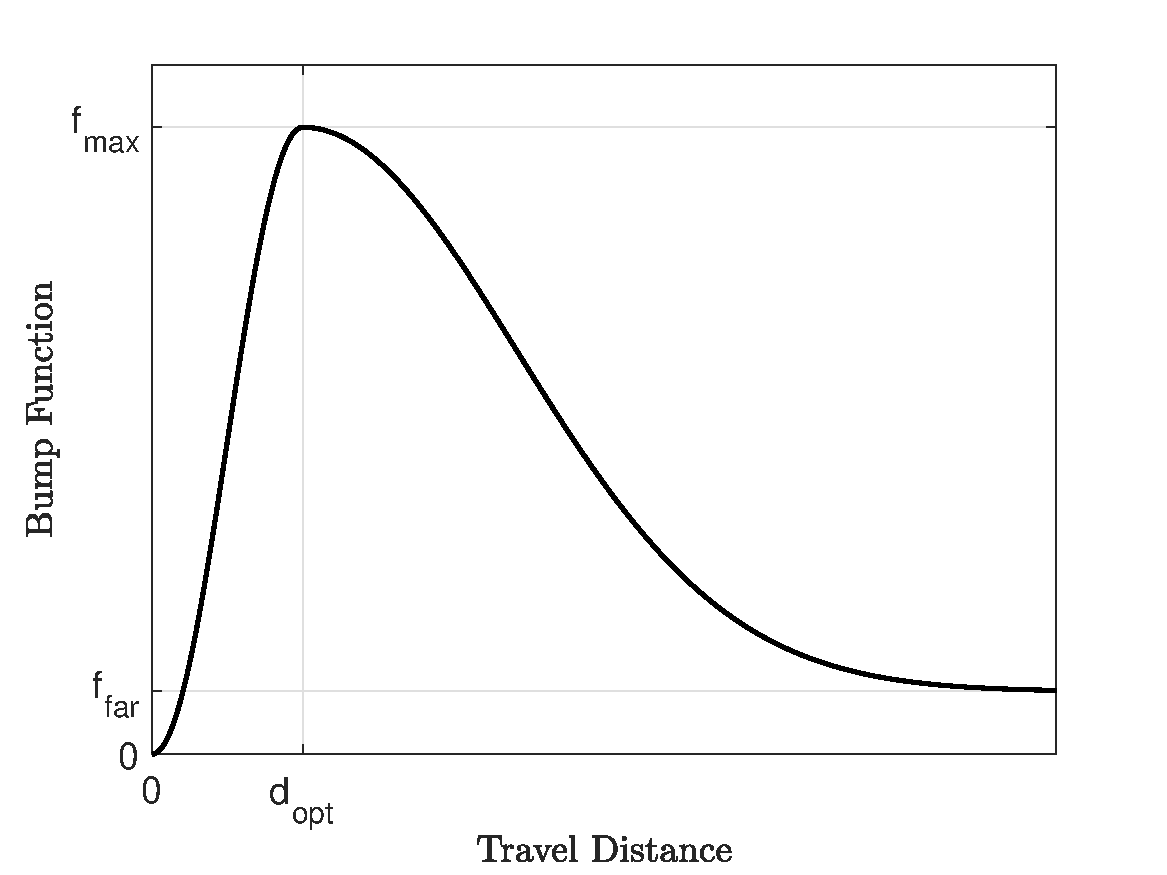
\includegraphics[width=0.9\columnwidth]{NonZeroBump.pdf}
		}
		\caption{The bump function is designed to promote travel distances close to $d_\text{opt}$ by multiplying this function by the expected information gain objective. Travel distances less than $d_\text{opt}$ are below the robot capabilities. Travel distances beyond $d_\text{opt}$ are beyond what the robot can reach within the minimum exploration computation time.}
		\label{fig:nonzeroBumpFun}
	\end{figure}
	
Then, using the information gain from \refeqn{expectedInfoGainMap2D} and considering the impact from travel distance from \refeqn{BumpFun}, the objective function for a single agent with respect to $X_{c}$ is
\begin{align}
\label{eqn:CandidateBidSingle}
\text{Obj}_\text{single}(X_k,X_c,m_\text{2D})&=\mathcal B(d(X_k,X_c,m_\text{2D}))\mathcal I(X_{c},m_\text{2D}).
%X_{k,c}^*&=\argmax_{X_c}{\ \mathcal B_{k,c}\mathcal I(X_c)},
\end{align}
Then, the optimal pose selection for the $k$-th agent is
\begin{align}
\label{eqn:OptPoseSingle}
X^*_{k}=\argmax_{X_c}\text{Obj}_\text{single}(X_k,X_c,m_\text{2D}).
\end{align}
Like \refeqn{BumpFunRef}, the bump function from \refeqn{BumpFun} prioritizes robotic movement within the local surrounding space before the robot moves across the map to distant regions, while still considering faraway pose candidates. Unlike \refeqn{BumpFunRef}, \refeqn{BumpFun} discourages the robot from staying motionless or near-motionless.

The first auction includes bids from all robots, and proceeds as follows. Let the set of all $n_R$ robots be denoted $\mathcal R=\braces{R_1,R_2,\dots,R_{n_R}}$ such that the $k$-th robot, namely $R_k$, bids $\text{Obj}_\text{single}(X^*_k,X_c,m_\text{2D})$ from \refeqn{CandidateBidSingle} and \refeqn{OptPoseSingle}. This is repeated for all $k$ such that $R_k\in\mathcal R$. The robot with the largest bid wins the first auction at index $k^*$, and is assigned to travel to $X^*_{k^*}$. Then, the remaining robots must account for the planned trajectory of the robot that won the first auction in subsequent auctions, described next.



\subsection{Objective Function for Subsequent Auctions}

The robots unable to win the first auction are updated to reflect the expected impact from the first robot traveling to optimal pose $X^*_{k^*}$.
This robot is expected to modify the probabilistic occupancy grid map, which may significantly change the expected information gains and collision properties of candidate poses nearby. The process of auctioning and modifying bids is repeated, removing the winning robot from consideration after each auction, until no robots remain. Between auctions, updating the map with expected measurements from auction-winning robots discourages the remaining robots from entering the same regions and capturing the same cells. As such, there is no need to consider the coverage overlap explicitly as in~\cite{SimApfBurFoxMooThrYou00}; instead coverage overlap is avoided in a systematic way as increased coverage overlap would reduce the overall information gain.

More specifically, we coordinate robotic efforts by modifying bids to prevent robots from updating the same grid cells and to avoid collisions among robots. The goal is to find the winning bids $\mathcal X^*=\braces{X^*_{1},X^*_{2},\dots,X^*_{n_R}}$ corresponding to each robot from $\mathcal R$. During the auctioning process, let $\mathcal W\subset\mathcal R$ be the set of robots that have already won auctions by producing the largest objective function bid. After the first auction described above, $\mathcal W=\braces{R_{k^*}}$; after all auctions are complete, $\mathcal W=\mathcal R$. Between auctions, the candidate poses are modified for information gain and collision-avoidance, coordinating the multi-vehicle exploration.

The first step between auctions is to modify the expected map information gain for efficient map coverage.  Once a robot wins a bid, the measurement ray expected values serve to update a temporary copy of $m_\text{2D}$, namely $m_\text{2D,copy}$, and those candidates located in a local neighborhood (twice the radius of a maximum sensor reading) of the winning candidate from the prior auction are recalculated, thereby coordinating total map information gain with auction-winning robots. Using the same local map notation from \refeqn{allEta} and \refeqn{Unnormalized} along a measurement ray, the expected measurement value is
\begin{align}
\label{eqn:ExpectedMeasRay}
\text{E}[z]=\sum_{k=1}^{n_{r}}\bigg\{\prod_{j=0}^{k-1}P(\bar{\mathbf{m}}_j)\bigg\}P(\mathbf{m}_k)z_k,
\end{align}
where $z_k$ denotes the distance from the robot sensor to the $k$-th cell along the measurement ray. Then $\text{E}[z]$ is substituted into \refeqn{RayISMAnswer}--\refeqn{allEta} to modify $m_\text{2D,copy}$, and expected map information gains are recomputed with \refeqn{ProbMeas} and \refeqn{expectedInfoGainRay}, while the bump function \refeqn{BumpFun} remains the same. In short, the expected changes of $m_\text{2D}$ are integrated into $m_\text{2D,copy}$ for expected information gain estimation between multiple vehicles.

% TODO: make sure find/replace of:
% \refeqn{RayISMAnswer}--\refeqn{Unnormalized}
%  \refeqn{RayISMAnswer}--\refeqn{allEta}

The second step focusses on collision-avoidance between robots based on their proximity. Let $\rho_\text{max}>0$ be a fixed maximum radius to consider collision-avoidance and $\rho_{i,c}\geq0$ be the Euclidean distance from the $i$-th already-assigned pose $X^*_i$ to the $c$-th candidate pose $X_c$, i.e.,
\begin{align}
\rho_{i,c}&=\norm{x^*_i-x_c},
\end{align}
where $x^*_i$ and $x_c$ are the pose locations of $X^*_i$ and $X_c$, respectively. Then the collision-avoidance factor for the $k$-th robot such that $R_k\notin\mathcal W$ is,
\begin{align}
\label{eqn:CollisionAvoidanceAmongRobots}
\mathbf C(X_c)&=
\begin{cases}
    \prod_{i|\mathcal{R}_i\in\mathcal W} \left(\frac{\rho_{i,c}}{\rho_\text{max}}\right)^2,		& \text{if }\rho_{i,c}<\rho_\text{max},\\
    1,              				& \text{otherwise},
\end{cases}
\end{align}
where this product serves to decrease the value of bids for candidate poses in close proximity with already-assigned poses to avoid collisions between robots. The multi-vehicle objective function for the $k$-th robot accounting for collision-avoidance is
\begin{align}
\label{eqn:CandidateBidMulti}
\text{Obj}_\text{multi}(X_k,X_c,m_\text{2D,copy})
=\mathbf C(X_c)\mathcal B(d(X_k,X_c,m_\text{2D}))\mathcal I(X_{c},m_\text{2D,copy}),
\end{align}
where its optimal pose during this auction is
\begin{align}
\label{eqn:OptPoseMulti}
X^*_{k}=\argmax_{X_c}\text{Obj}_\text{multi}&(X_k,X_c,m_\text{2D,copy}),
\end{align}
such that $\text{Obj}_\text{multi}(X^*_k,X_c,m_\text{2D,copy})$ is the bid for the $k$-th robot.
Optimal pose selection and bidding is repeated for all robots not belonging to $\mathcal W$. The largest bid among these wins the auction and is tasked with moving to the associated pose candidate, and then this robot is included with $\mathcal W$ to avoid further consideration. Completing $n_R$ auctions produces the set of coordinated poses $\mathcal X^*$.

The proposed approach uses auctions and bid modifications based on total map expected information gain and collision-avoidance, promoting exploration of different spaces without explicit consideration of coverage overlaps. The pseudocode for the bidding process is shown with Algorithm \ref{alg:bidding}.

\begin{algorithm}
	Function: $Bidding(\mathcal X_r,\mathcal I(X_c)\forall c\in\mathcal C,\rho_\text{max})$\;
	Initialize $k=0$, $\mathcal W=0_{n_R\times1}$, $B=0_{n_R\times1}$\;
	Update candidate expected information gains using \refeqn{DiscExpEntropyRay}\;
	\For{$i=n_R,n_R-1,\ldots,1$}{
		\For{$j=1,2,\ldots,n_R$}{
			\If{$\mathcal W(j)==0$}{
				\If{$i==n_R$}{
					Maximize bid \refeqn{CandidateBidSingle} for $X^*_{j}$ from \refeqn{OptPoseSingle}\;
				}
				\Else{
					Update $\mathcal I(X_c)$ close to $\mathcal X^*(k)$\;
					\For{$c=1,2,\ldots,n_c$}{
						Find Euclidean distance $\rho_{k,c}$\;
					Get $\mathbf C(X_c)$ with \refeqn{CollisionAvoidanceAmongRobots}\;
					}
					Maximize bid \refeqn{CandidateBidMulti} for $X^*_{j}$ from \refeqn{OptPoseMulti}\;
				}
				Insert the $j$-th maximum bid into $B(j)$\;
			}
		}
		$k$: index maximizing $B$ with corresponding $X^*_{k}$\;
		$\mathcal X^*(k)=X^*_{k}$\;
		$\mathcal W(k)=1$\;
		$B(k)=0$\;
	}

	Return $\mathcal X^*$\;
\caption{Robot Task Bidding}
\label{alg:bidding}
\end{algorithm}


\subsection{Receding Horizon Framework}

This algorithm is further aided by following a receding horizon framework for improved information gain maximizations and collision-avoidance with dynamic obstacles and other robots. A receding horizon simply repeats the autonomous exploration steps as quickly as possible over a finite time period, frequently before a robot reaches its desired pose. Since exploration optimizations can only occur during exploration updates, a receding horizon maximizes the rate at which these updates occur. These updates require time for computation, over which the robot can move $d_\text{opt}$, used to optimize the robot travel distances with \refeqn{BumpFun}. Hence, the receding horizon framework serves to repeat optimizations as quickly as possible with maximal robotic movement while exploring a changing occupancy grid.

Furthermore, a receding horizon framework enhances autonomous exploration in two other ways. First, the occupancy grid map is constantly updated while a robot traverses a trajectory, so the expected information gains change as well. Since the bids depend on the occupancy grid, $\mathcal X^*$ is updated accordingly. This prevents robots from completing trajectories that have become unnecessary as new terrain becomes captured. Second, the receding horizon prevents robots from colliding with each other when they become too close together (e.g., crossing paths, traversing a tight passage) or other moving obstacles (e.g., a human). The cost map for each robot is updated, and the location of other robots are considered as collision-prone space. Hence, the robot trajectories become better separated due to rapid updates of the cost maps with the receding horizon. 

\subsection{Multi-Vehicle Exploration Numerical Simulation}
% Multi-vehicle ICRA figs 3-6 (remake fig. 5 with larger contrast)

\section{Multi-Vehicle Cooperative Patrol}

\subsection{Continuous-Time Markov Process for Cell Degradation}
% JINT18 fig. 3

\subsection{Multi-Vehicle Patrol Numerical Simulation}
% JINT18 fig. 10-13 (ref. ICRA fig 3 from above in this chapter)

\section{Conclusions}





